\paragraph{} Esta es la página del administrador para modificar elementos en la base de datos de una manera sencilla. Aquí se muestra al administrador un formulario con un campo por característica del microcontrolador, con la información actual sobre el mismo ya cargada, y que el administrador puede modificar a su gusto.
\begin{itemize}
\item \textbf{Arquitectura}
\item \textbf{Frecuencia(MHz)}
\item \textbf{Flash(Kb})
\item \textbf{RAM(Kb}) 
\item \textbf{Precio($\euro$)}
\end{itemize}

\paragraph{} El campo \textbf{''Referencia''} no será editable.

\paragraph{} Al pulsar el botón situado a la derecha se modifica el elemento en la base de datos y automáticamente se redirigirá al administrador a la página de listado completo, con el nuevo microcontrolador ya incluido en la lista.

\begin{figure}[h!]
	\centering
	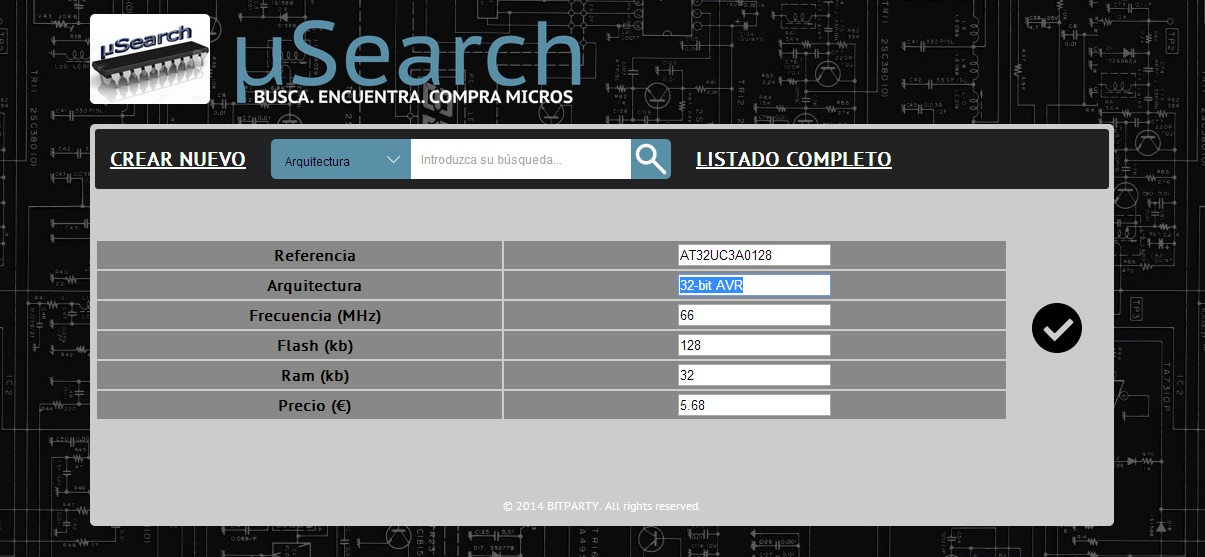
\includegraphics[width=0.85\textwidth]{img/editar}
	\caption{Página para modificar un micro-controlador.}
	\label{fig:editar}
\end{figure}

\paragraph{}Como en todas las demás páginas del sitio web, si se pulsa en cualquiera de los dos logotipos del catálogo $\mu$Search (esquina superior izquierda), el sistema redirigirá al administrador a la página inicial de administración del catálogo.

\paragraph{}Además, desde esta página de edición, a través de los iconos situados en la cabecera debajo de los logotipos de la web, el administrador puede acceder a:

\begin{itemize}
	\item \textbf{Crear Nuevo:} Pulsando sobre este botón el administrador es redirigido a la página que le permitirá añadir un nuevo microcontrolador a la base de datos del catálogo electrónico.

	\item \textbf{Búsqueda:} Desde esta sección de la cabecera, el administrador puede realizar búsquedas sobre el catálogo de microcontroladores en base a cualquiera de las diferentes características de un microcontrolador (Arquitectura, Frecuencia, Flash, RAM). Simplemente se debe seleccionar una de las características de la lista despegable, introducir el texto a buscar y pulsar sobre el icono de búsqueda.
	El administrador será redirigido a una página donde se le mostrará el resultado de la búsqueda en forma de lista de microcontroladores.
			
	\item \textbf{Listado Completo:} Pulsando sobre este botón/icono el sistema redirige al administrador a la página en la que se listan todos los elementos disponibles en el catálogo de microcontroladores.
\end{itemize}